\section{Mangel på samtidighed}\label{rel:samtidighed}

\subsection{Synkronisering af ure} \label{sec:sync}

\begin{figure}
    \centering
    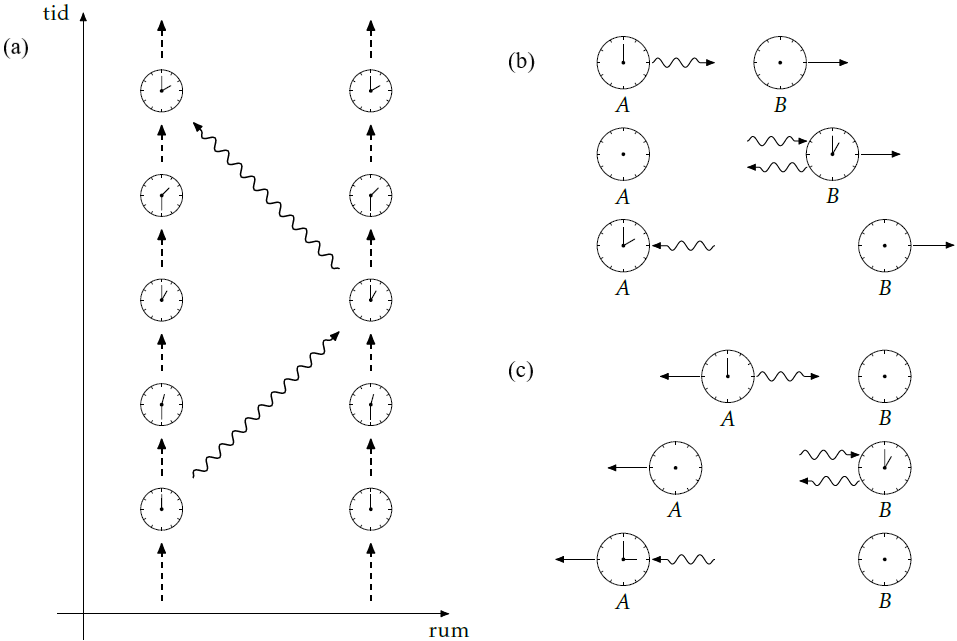
\includegraphics[width=0.85\textwidth]{SR/billeder/EinsteinSynkronisering.png}
    \caption{Einsteinsynkronisering. a) Ved at sende informationer om urenes
visning frem og tilbage ved brug af lyssignaler, kan det afgøres om urene er synkroniserede. b) Forsøg på synkronisering mens ur B er i bevægelse væk fra ur A. c) Forsøg på synkronisering mens ur A er i bevægelse væk fra ur B. \newline Kilde: figur~3.1 og 3.2 i \cite{uggerhojSpecielRelativitetsteori2016}.}
    \label{fig:EinsteinSyncornization}
\end{figure}

Vi kan forestille os, at vi ønsker at synkronisere to ure, så to forskellige personer kan være enige om tiden. Dette kan gøres ved at sende et lysglimt indeholdende information omkring afsendingstidspunktet fra ur A til ur B. Lige ved modtagelsen af lysglimtet afsendes et nyt lysglimt, indeholdende information omkring dettes afsendingstidspunkt, fra ur B til ur A. Når dette lysglimt når ur A sammenlignes afsendingstidspunktet for lysglimtet fra ur B med tidspunktet for afsendingen af det første lysglimt fra ur A og modtagelsen af lysglimtet fra ur B, se figur \ref{fig:EinsteinSyncornization}a. Befinder afsendingstidspunktet for lysglimtet fra ur B sig midt mellem de to andre tidspunkter, da er urene synkroniserede. Eksempelvis: Ur A afsender kl. 12.00 et lysglimt til ur B, som modtager dette kl. 13.00 og straks sender et lysglimt tilbage til ur A, som modtager dette kl. 14.00. Kl. 13.00 ligger midt mellem kl. 12.00 og kl. 14.00, hvorfor de to ure er synkroniserede. Denne metode til synkronisering af ure kaldes for \textit{Einsteinsynkronisering}. Dette gør sig gældende for ure, der enten er stillestående eller i ens bevægelse, men ikke for ure i indbyrdes (relativ) bevægelse. Dette kan ses ved at benytte samme opstilling som før, blot hvor det ene ur er i bevægelse i forhold til det andet. Er ur B i bevægelse væk fra ur A, figur \ref{fig:EinsteinSyncornization}b, da vil lysglimtet stadig tilbagelægge den samme vejlængde frem og tilbage, hvorfor samme konklusion som ovenfor fås, at urene \emph{er} synkroniserede. Er ur A derimod i bevægelse væk fra ur B, figur \ref{fig:EinsteinSyncornization}c, da vil lysglimtet fra ur B til ur A have længere vej at tilbagelægge end lysglimtet fra ur A til ur B, hvorfor afsendingstidpunktet for lysglimtet fra ur B ikke vil ligge midt mellem afsendings- og modtagningstidspunkterne ved ur A. Ud fra proceduren kan der derved konkluderes, at de to ure \emph{ikke} er synkroniserede. Men ser man på det tilfældet, hvor ur B bevæger sig væk fra ur A, blot fra ur B's synspunkt, da ses ur B som værende stationært, mens ur A bevæger sig væk fra ur B, altså at de to tilfælde -- figur \ref{fig:EinsteinSyncornization}b og \ref{fig:EinsteinSyncornization}c -- er ens, blot set fra forskellige hvilesystemer. Ifølge relativitetsprincippet må synkroniseringen ikke afhænge af, om man ser situationen fra det ene eller det andet hvilesystem, hvorfor det må konkluderes, at to ure i indbyrdes bevægelse ikke kan synkroniseres.

En anden måde at se at synkronisering af ure i indbyrdes bevægelse ikke er mulig er, at huske tilbage til afsnit \ref{sec:Tidsforlaengelse}, hvor vi så, at ''et ur i bevægelse går langsomt''. Så selvom de to ure kunne synkroniseres, da ville overensstemmelsen gå tabt med det samme, da urene bevæger sig med forskellig hastighed, hvilket resulterer i samme konklusion som ovenfor.


\subsection{Einsteins togeksperiment} \label{sec:tog}

For at beskrive manglen på samtidighed lidt mere visuelt gøres brug af et tankeeksperiment kaldet \emph{Einsteins togeksperiment}. Einsteins togeksperiment består af to personer, Fulbert og Beatrice, og to ure. Fulbert er placeret på en togperron midt mellem de to stillestående ure, der er synkroniserede, mens Beatrice er placeret midt i toget, der kører forbi perronen. Afstanden mellem urene er præcis sådan, at idet Fulbert og Beatrice er lige ud for hinanden, da vil togets for- og bagende være præcist ud for hvert deres ur. På nøjagtig dette tidspunkt, f.eks. kl. 12.00, udsendes et lysglimt, en refleksion af lyset fra urskiven da viserne viste nøjagtigt kl. 12.00, fra hvert af urene mod Fulbert og Beatrice. Fulbert modtager begge lysglimt samtidig og konkluderer da, at lysglimtene blev udsendt samtidig, altså at urene er synkroniserede. I løbet af den tid der går, fra lysglimtene bliver afsendt fra urene, og til lysglimtene krydser hinanden ved Fulbert, har toget med Beatrice bevæget sig fremad, se figur \ref{fig:EinsteinsTrainExperiment}. Lysglimtene mødes altså ikke i midten af toget, men tættere på bagenden af toget. Selvom Fulbert ser de to glimt som værende afsendt samtidig, da vil Beatrice konkludere, at lysglimtet fra uret ved togets forende er afsendt først, da dette lysglimt visende kl. 12.00 blev set først i toget, hvorefter lysglimtet fra det andet ur, også visende kl. 12.00, blev set, og Beatrice var placeret midt mellem de to ure, da lysglimtet blev udsendt.
%
\begin{figure}[t]
    \centering
    \begin{subfigure}[t]{.3\textwidth}
        \centering
        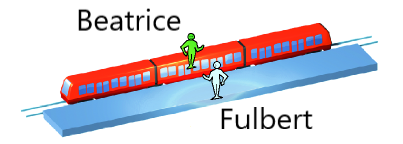
\includegraphics[width=\columnwidth]{SR/billeder/EinsteinTrainExperiment1.PNG}
        \caption{Fulbert er placeret midt på en togperron, og Beatrice er placeret midt i et forbikørende tog.}
        \label{fig:EinsteinsTrainExperiment1}
    \end{subfigure}
    \hfill
    \begin{subfigure}[t]{.3\textwidth}
        \centering
        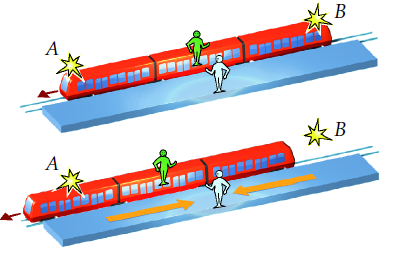
\includegraphics[width=\columnwidth]{SR/billeder/EinsteinTrainExperiment2.PNG}
        \caption{Fra Fulberts perspektiv udsendes lysglimtene samtidig i togets for- og bagende (punkt A og B).}
        \label{fig:EinsteinsTrainExperiment2}
    \end{subfigure}
    \hfill
    \begin{subfigure}[t]{.3\textwidth}
        \centering
        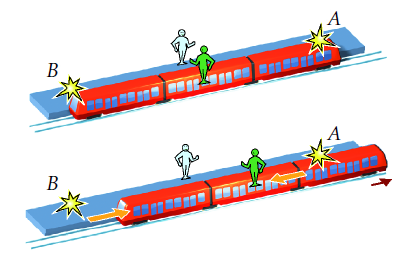
\includegraphics[width=\columnwidth]{SR/billeder/EinsteinTrainExperiment3.PNG}
        \caption{Idet Beatrice (og dermed toget) bevæger sig mod punkt A, vil hun opleve, at lysglimetet, der blev udsendt fra togets forende, blev udsendt før det i togets bagende, idet lyset bevæger sig med samme hastighed fra de to lysglimt.}
        \label{fig:EinsteinsTrainExperiment3}
    \end{subfigure}
    \caption{Einsteins togeksperiment. Kilde: \cite{uggerhojSpecielRelativitetsteori2016}.}
    \label{fig:EinsteinsTrainExperiment}
\end{figure}
%
Da Beatrice modtager signalet fra ur A før hun modtager signalet fra ur B
% Set fra Beatrices perspektiv viser ur A -- det for hende bagerste perronur, da Beatrice ser perronen med Fulbert og urene bevæge sig den modsatte retning af, hvad Fulbert ser toget bevæge sig -- kl. 12.00 og først lidt senere viser ur B -- det for hende forreste perronur -- kl. 12.00. Beatrice 
konkluderer hun, at ur A er tidsmæssigt foran, hvorimod Fulbert konstaterede at de var synkroniserede. \\
Konklusionen er, at begivenheder, der sker samtidigt for Fulbert, ikke nødvendigvis gør det for Beatrice. Dette kan opsummeres som:
\begin{quote}
	Begivenheder, der sker på samme \textit{tid}, men på forskellige \textit{steder} for én observatør, sker til forskellige \textit{tider} for en observatør, der er i bevægelse i forhold til den første.
\end{quote}
I relativitetsteori behandles tid og rum på (næsten) lige fod, og benyttes nu denne lighed kan ovenstående sætning direkte omskrives til:
\begin{quote}
	Begivenheder der sker på samme \textit{sted}, men til forskellige \textit{tider} for én observatør, sker på forskellige \textit{steder} for en observatør, der er i bevægelse i forhold til den første.
\end{quote}
Dette beskriver netop manglen på absolut samtidighed.